%%%%%%%%%%%%%%%%%%%%%%%%%%%%%%%%%%%%%%%%%
% Beamer Presentation
% LaTeX Template
% Version 1.0 (10/11/12)
%
% This template has been downloaded from:
% http://www.LaTeXTemplates.com
%
% License:
% CC BY-NC-SA 3.0 (http://creativecommons.org/licenses/by-nc-sa/3.0/)
%
%%%%%%%%%%%%%%%%%%%%%%%%%%%%%%%%%%%%%%%%%

%----------------------------------------------------------------------------------------
%	PACKAGES AND THEMES
%----------------------------------------------------------------------------------------

\documentclass{beamer}

\mode<presentation> {

% The Beamer class comes with a number of default slide themes
% which change the colors and layouts of slides. Below this is a list
% of all the themes, uncomment each in turn to see what they look like.

%\usetheme{default}
%\usetheme{AnnArbor}
%\usetheme{Antibes}
%\usetheme{Bergen}
%\usetheme{Berkeley}
%\usetheme{Berlin}
%\usetheme{Boadilla}
%\usetheme{CambridgeUS}
%\usetheme{Copenhagen}
%\usetheme{Darmstadt}
\usetheme{Dresden}
%\usetheme{Frankfurt}
%\usetheme{Goettingen}
%\usetheme{Hannover}
%\usetheme{Ilmenau}
%\usetheme{JuanLesPins}
%\usetheme{Luebeck}
%\usetheme{Madrid}
%\usetheme{Malmoe}
%\usetheme{Marburg}
%\usetheme{Montpellier}
%\usetheme{PaloAlto}
%\usetheme{Pittsburgh}
%\usetheme{Rochester}
%\usetheme{Singapore}
%\usetheme{Szeged}
%\usetheme{Warsaw}

% As well as themes, the Beamer class has a number of color themes
% for any slide theme. Uncomment each of these in turn to see how it
% changes the colors of your current slide theme.

%\usecolortheme{albatross}
%\usecolortheme{beaver}
%\usecolortheme{beetle}
%\usecolortheme{crane}
%\usecolortheme{dolphin}
%\usecolortheme{dove}
%\usecolortheme{fly}
%\usecolortheme{lily}
%\usecolortheme{orchid}
%\usecolortheme{rose}
%\usecolortheme{seagull}
%\usecolortheme{seahorse}
%\usecolortheme{whale}
%\usecolortheme{wolverine}

%\setbeamertemplate{footline} % To remove the footer line in all slides uncomment this line
%\setbeamertemplate{footline}[page number] % To replace the footer line in all slides with a simple slide count uncomment this line

%\setbeamertemplate{navigation symbols}{} % To remove the navigation symbols from the bottom of all slides uncomment this line
}

\usepackage{listings}
\usepackage{color}

\usepackage{hyperref}
 
\definecolor{codegreen}{rgb}{0,0.6,0}
\definecolor{codegray}{rgb}{0.5,0.5,0.5}
\definecolor{codepurple}{rgb}{0.58,0,0.82}
\definecolor{backcolour}{rgb}{0.95,0.95,0.92}
 
\lstdefinestyle{mystyle}{
    backgroundcolor=\color{backcolour},   
    commentstyle=\color{codegreen},
    keywordstyle=\color{magenta},
    numberstyle=\tiny\color{codegray},
    stringstyle=\color{codepurple},
    basicstyle=\footnotesize, %\tiny, \small, \footnotesize
    breakatwhitespace=false,         
    breaklines=true,                 
    captionpos=b,                    
    keepspaces=true,                 
    numbers=left,                    
    numbersep=5pt,                  
    showspaces=false,                
    showstringspaces=false,
    showtabs=false,                  
    tabsize=2
}
 
\lstset{style=mystyle}

\usepackage{hyperref}
\usepackage{lipsum}
\usepackage{graphicx} % Allows including images
\usepackage{booktabs} % Allows the use of \toprule, \midrule and \bottomrule in tables

%My personal package
%\usepackage{tikz}
\usepackage{amsmath,nccmath}
%\usepackage{media9}
%\usepackage{multimedia}
\usepackage{xmpmulti}

%% Knuths smile box from 
%\centerline{\bf Stable Husbands}
%\bigskip
%\centerline{\sl Donald E. Knuth, Rajeev Motwani, and Boris Pittel}
%\centerline{\sl  Computer Science Department, Stanford University}
\def\pfbox % new experimental version (DEK, November 88)
{{\ooalign{\hfil\lower.06ex % a smiley face
 \hbox{$\scriptscriptstyle -$}\hfil\crcr
 \hfil\lower.7ex\hbox{\"{}}\hfil\crcr
 \mathhexbox20D}}}

%----------------------------------------------------------------------------------------
%	TITLE PAGE
%----------------------------------------------------------------------------------------

\title[CFD]{ENT441 Computational Fluid Dynamics} % The short title appears at the bottom of every slide, the full title is only on the title page

\author{Muhammad Izham, PhD} % Your name
\institute[Universiti Malaysia Perlis] % Your institution as it will appear on the bottom of every slide, may be shorthand to save space
{
Universiti Malaysia Perlis \\ % Your institution for the title page
\medskip
\textit{izham@unimap.edu.my} \\
\textit{sugita5019@gmail.com} \\ %email

%Check out my templates for simple stuffs

\href{https://github.com/izham-sugita}{https://github.com/izham-sugita}

%\href{http://www.latex-tutorial.com}{LaTeX-Tutorial}.
}
\date{} % Date, can be changed to a custom date

\begin{document}

\begin{frame}
\titlepage % Print the title page as the first slide
\end{frame}

\begin{frame}[fragile]
\frametitle{Why Computational Fluid Dynamics?}
\begin{figure}

\includegraphics[width=0.8\linewidth]{./image/isaacnewton1-2x}
\end{figure}
\end{frame}


\begin{frame}[fragile]
\frametitle{COLORFUL FLUID DYNAMICS }
\begin{figure}
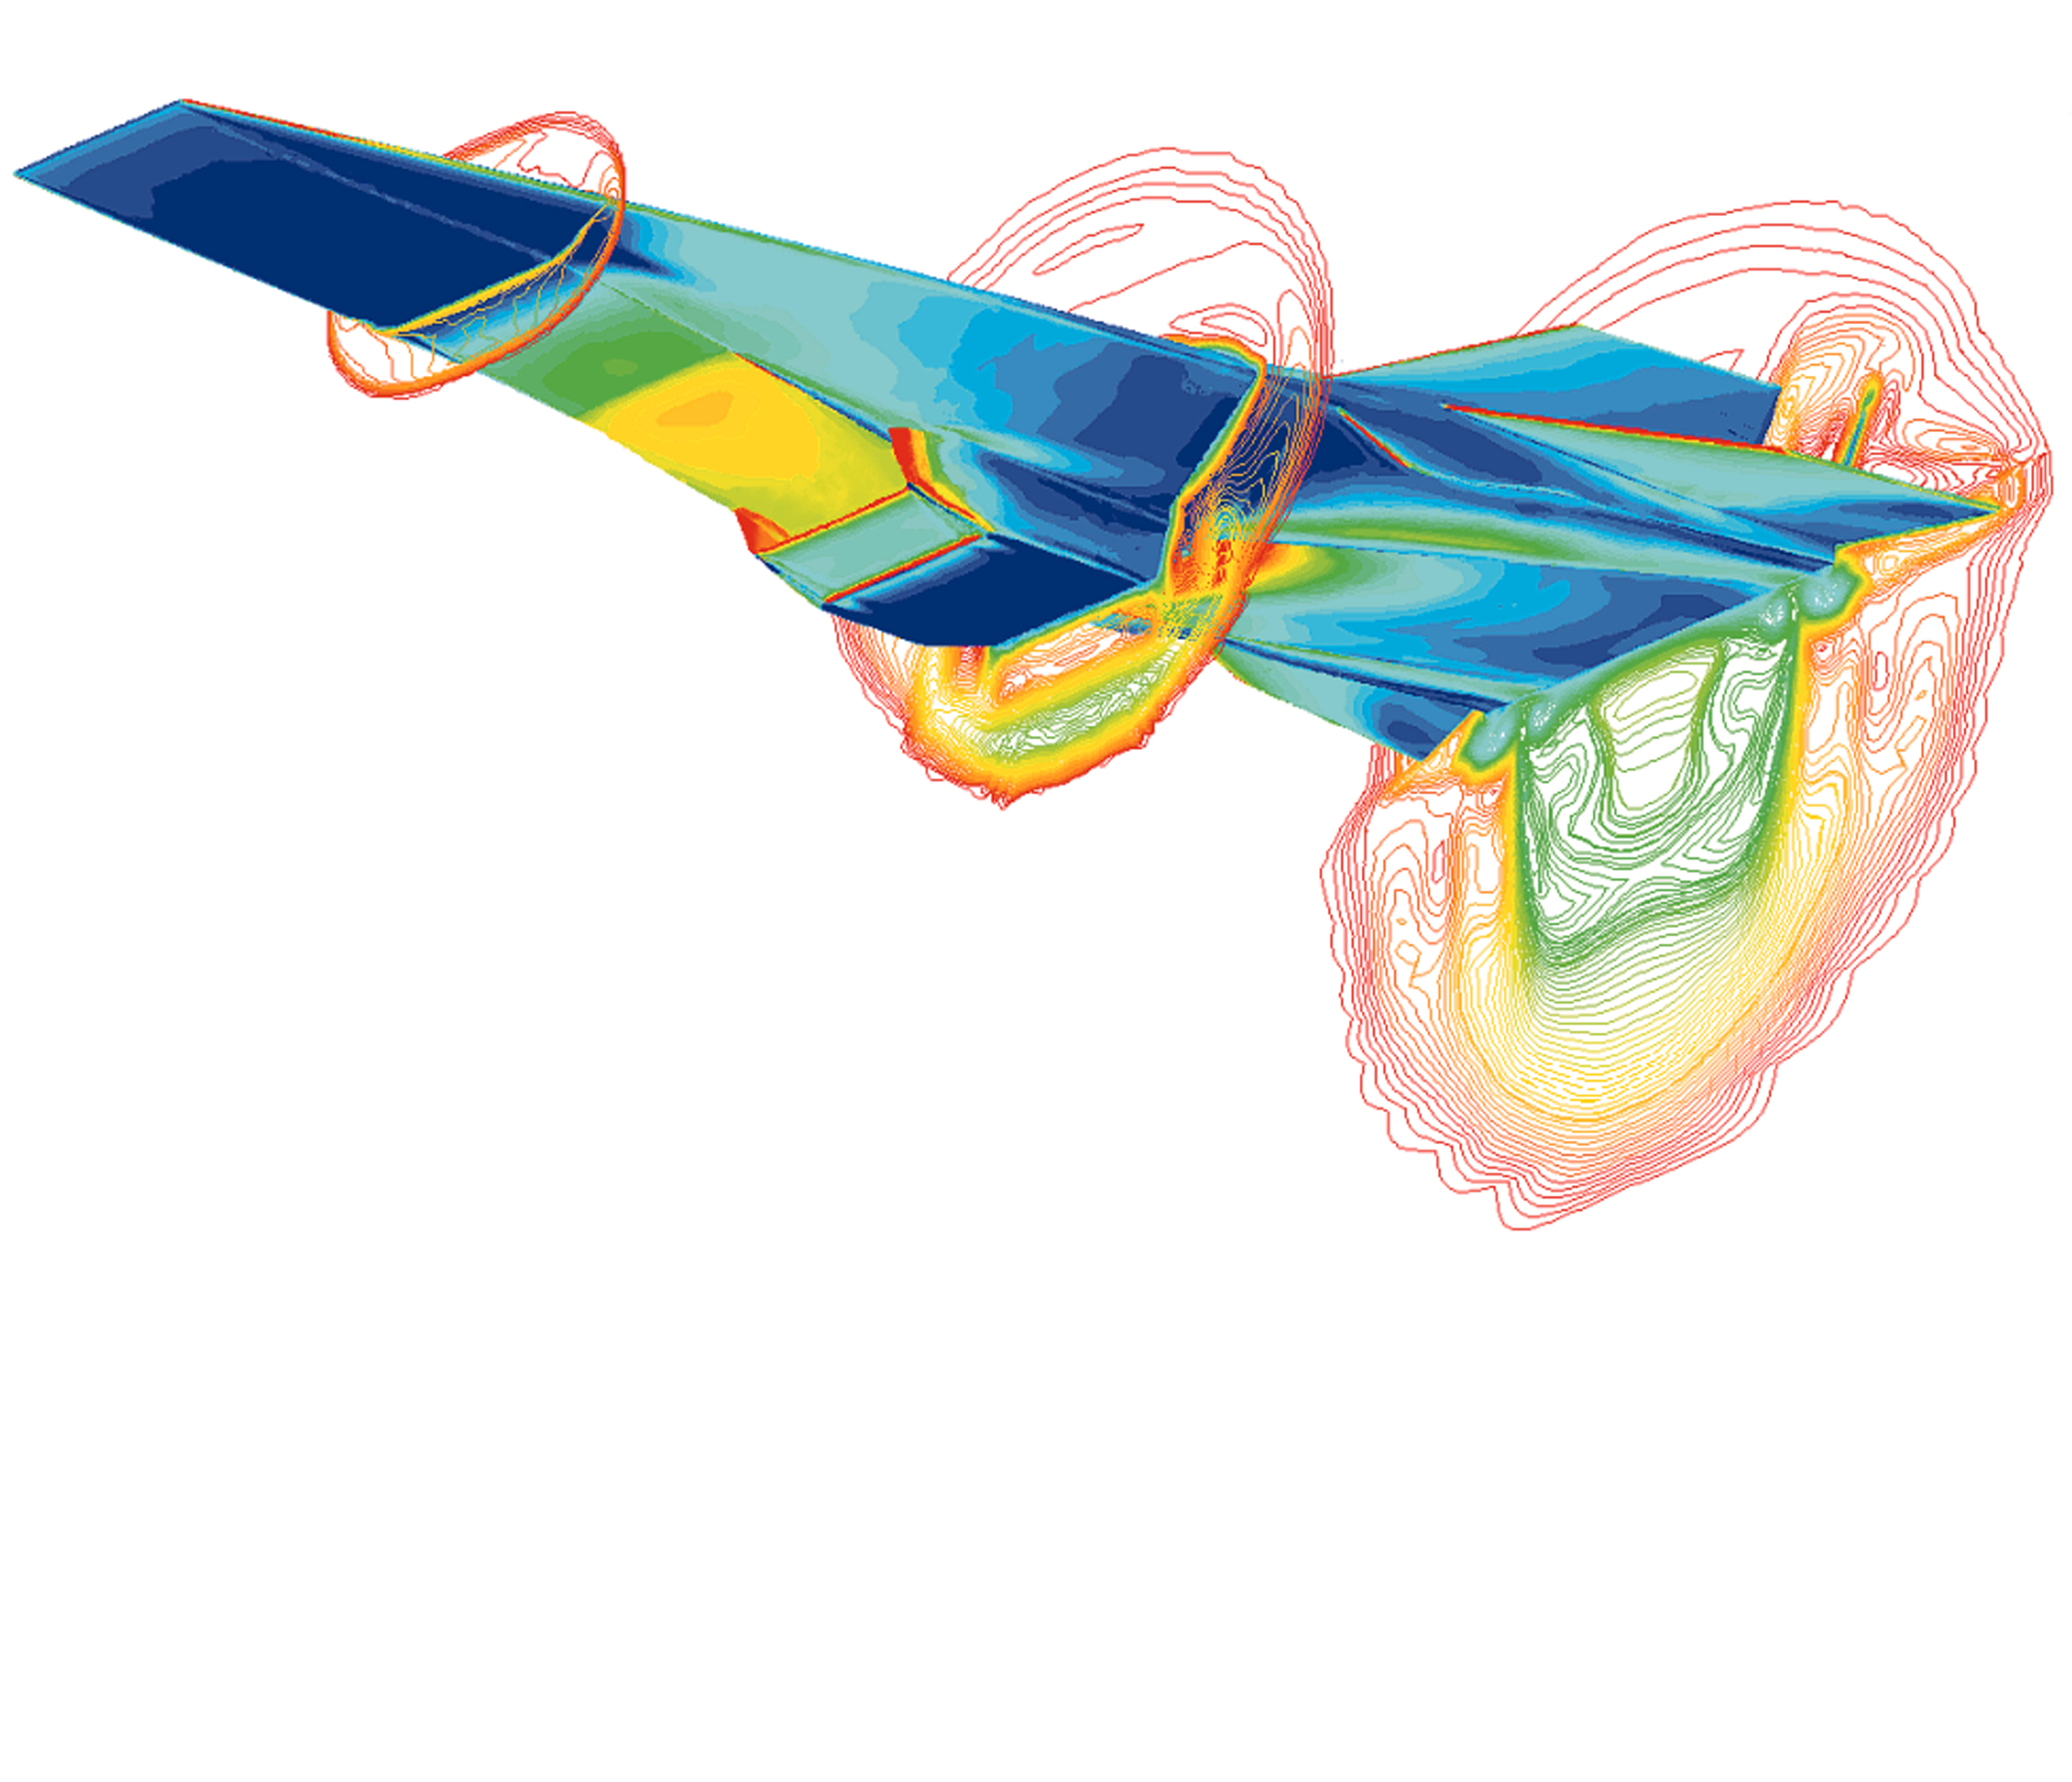
\includegraphics[width=0.75\linewidth]{./image/hyperX-1}
\end{figure}
\end{frame}



\begin{frame}
\frametitle{Overview} % Table of contents slide, comment this block out to remove it
\tableofcontents % Throughout your presentation, if you choose to use \section{} and \subsection{} commands, these will automatically be printed on this slide as an overview of your presentation
\end{frame}

%----------------------------------------------------------------------------------------
%	PRESENTATION SLIDES
%----------------------------------------------------------------------------------------

\section{Model Partial Differential Equations}
\subsection{Advection Equation}
\newcounter{test}
\newcommand\AdvecTitle{%
  \frametitle{\refstepcounter{test} Advection equation~\thetest}}
\resetcounteronoverlays{test}


\begin{frame}[fragile]
%\frametitle{Advection equation}
\AdvecTitle
\begin{itemize}
\item Linear advection equation.
      \begin{fleqn}
      \begin{equation}
      \frac{\partial u}{\partial t} + c \frac{\partial u}{\partial x} = 0, \qquad
      c \geq 0
      \label{eq:advection}
      \end{equation}
      
      \begin{equation}
      u\left(x,0\right)=u_0 \nonumber
      \label{eq:advection}
      \end{equation}
      \end{fleqn}
\end{itemize}
\end{frame}

\begin{frame}[fragile]
%\frametitle{Advection equation}
\AdvecTitle
\begin{itemize}
\item Initial condition and analytical solution at t=2.0000.
	  \begin{fleqn}
      \begin{equation}
      u_0 = \begin{cases} 1.0 \qquad 2.0 \leqslant x \leqslant 4.0 \\ 0.0 \qquad other \end{cases} \nonumber
      \end{equation}
      \end{fleqn} 

\begin{figure}
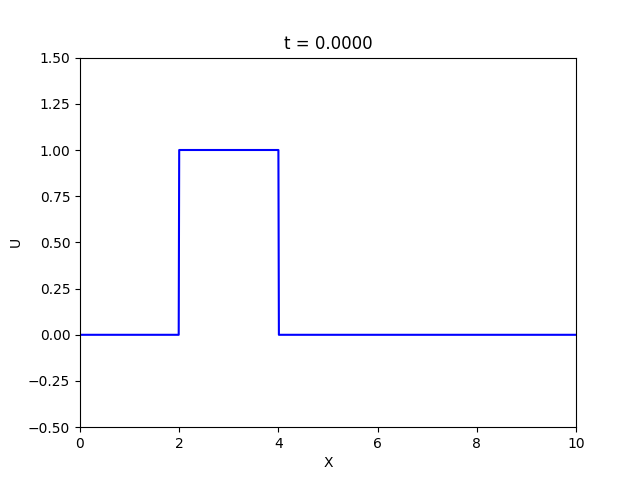
\includegraphics[width=0.5\textwidth, height=0.25\textwidth]{./image/init.png}%
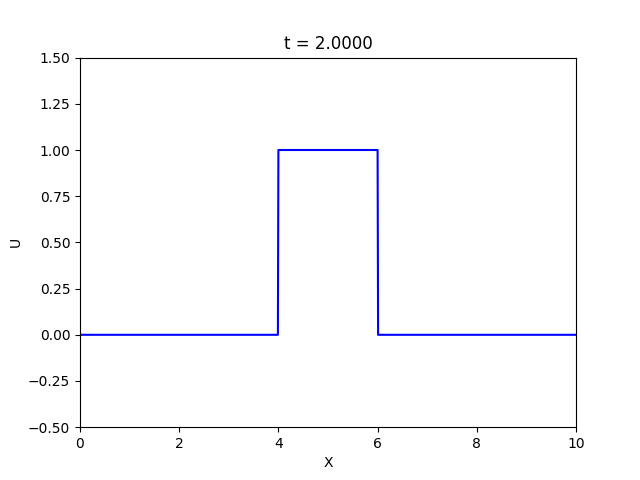
\includegraphics[width=0.5\textwidth, height=0.25\textwidth]{./image/final.png}
\caption{Left is at t=0.0000 and right is at t=2.0000}
\end{figure}

\end{itemize}
\end{frame}


\begin{frame}[fragile]
\AdvecTitle
\begin{itemize}
\item Sample of upwind discretization in Python.
\lstinputlisting[language=Python, firstline=1, lastline=2]{./codes/upwind.py}
\lstinputlisting[language=Python, firstline=27, lastline=36]{./codes/upwind.py}

\end{itemize}

\end{frame}

\subsection{Diffusion/Heat Equation} 
\newcounter{counter}
\newcommand\DiffTitle{%
  \frametitle{\refstepcounter{counter} Diffusion/Heat equation~\thecounter}}
\resetcounteronoverlays{counter}


\begin{frame}[fragile]
\DiffTitle
\begin{itemize}
\item Diffusion equation or heat equation.
      \begin{fleqn}
      \begin{equation}
      \frac{\partial T}{\partial t} = \kappa \frac{\partial^2 T}{\partial x^2}
      \label{eq:heat}
      \end{equation}
      \end{fleqn}

\item The boundary condition
\begin{fleqn}
      \begin{equation}
       T\left(x,0\right) = \begin{cases} f\left(x\right) \qquad Neumann \ BC \\ 
      const. \qquad Dirichlet \ BC \end{cases} \qquad \forall x \in \left[0,L\right]
      \end{equation}
      \end{fleqn}      
      
\end{itemize}
\end{frame}

\begin{frame}[fragile]
\DiffTitle
\begin{itemize}
\item Diffusion/Heat equation in one-dimension
\begin{figure}
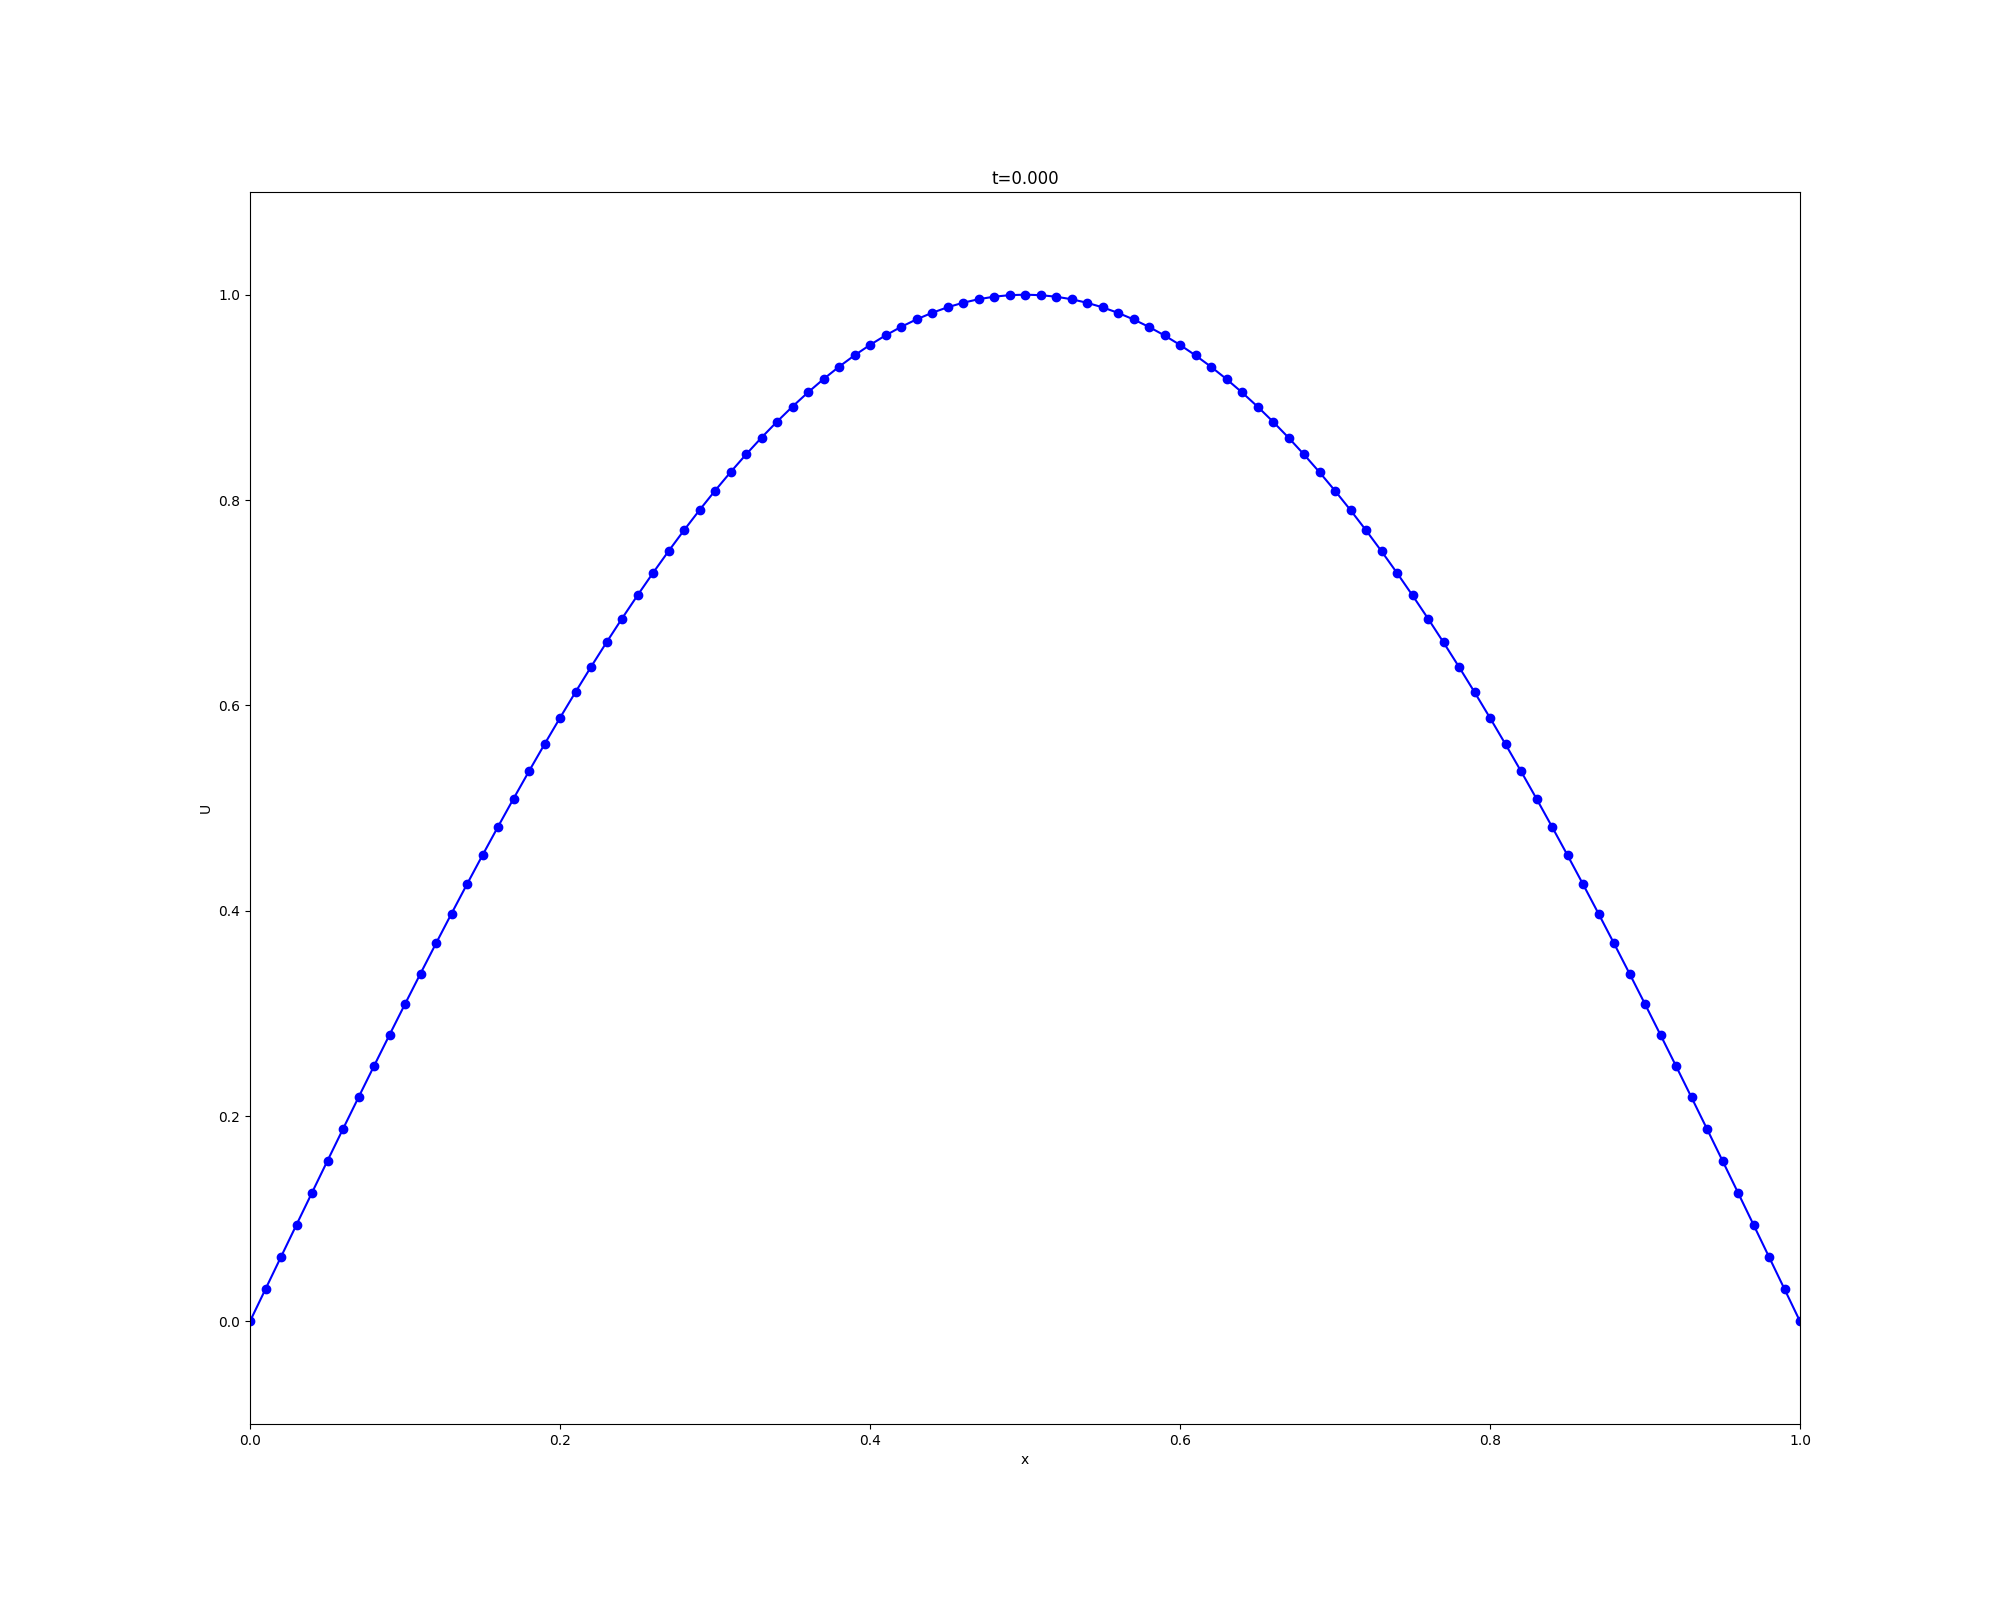
\includegraphics[width=0.5\textwidth, height=0.25\textwidth]{./image/diff_init.png}%
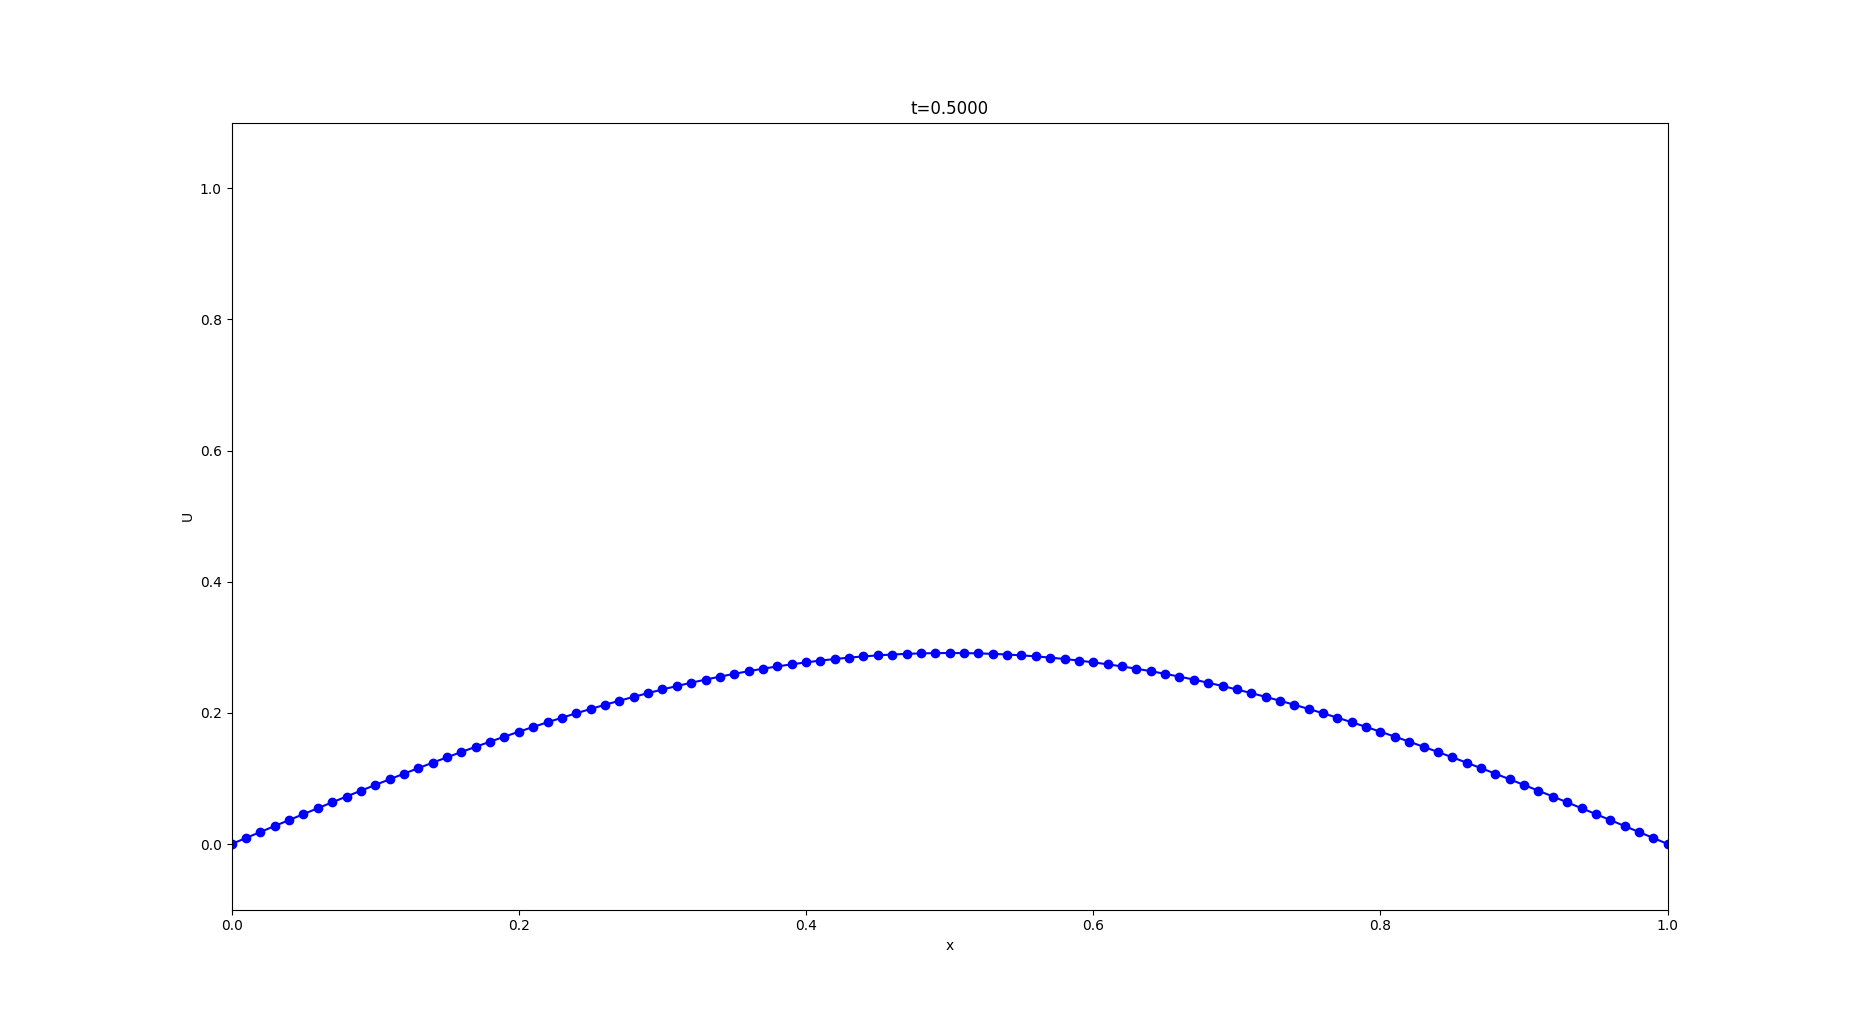
\includegraphics[width=0.5\textwidth, height=0.25\textwidth]{./image/diff_final.png}
\caption{Left is at t=0.0000 and right is at t=0.5000}
\end{figure}
\end{itemize}
\end{frame}

\begin{frame}[fragile]
\DiffTitle
\begin{itemize}
\item Sample of the heat equation discretization in Python.
\lstinputlisting[language=Python, firstline=47, lastline=57]{./codes/heat1D.py}
\end{itemize}
\end{frame}

\subsection{Poisson Equation} 
\newcounter{count}
\newcommand\PoissonTitle{%
  \frametitle{\refstepcounter{count} Poisson/Laplace equation~\thecount}}
\resetcounteronoverlays{count}


\begin{frame}[fragile]
\PoissonTitle
\begin{itemize}
\item Poisson equation/ Laplace equation.
      \begin{fleqn}
      \begin{equation}
      -\frac{\partial^2 u}{\partial x^2} = \begin{cases} f\left(x\right) \qquad Poisson \ equation \\ 
      0 \qquad \qquad Laplace \ equation \end{cases} \qquad \forall x \in \left[0,L\right]
      \label{eq:poisson}
      \end{equation}
      \end{fleqn}

\item The boundary condition
\begin{fleqn}
      \begin{equation}
       T\left(x,0\right) = \begin{cases} g\left(x\right) \qquad Neumann \ BC \\ 
      const. \qquad Dirichlet \ BC \end{cases} \qquad \forall x \in \left[0,L\right]
      \end{equation}
      \end{fleqn}      
      
\end{itemize}
\end{frame}

\begin{frame}[fragile]
\PoissonTitle
\begin{itemize}
\item Diffusion/Heat equation in one-dimension
\begin{figure}
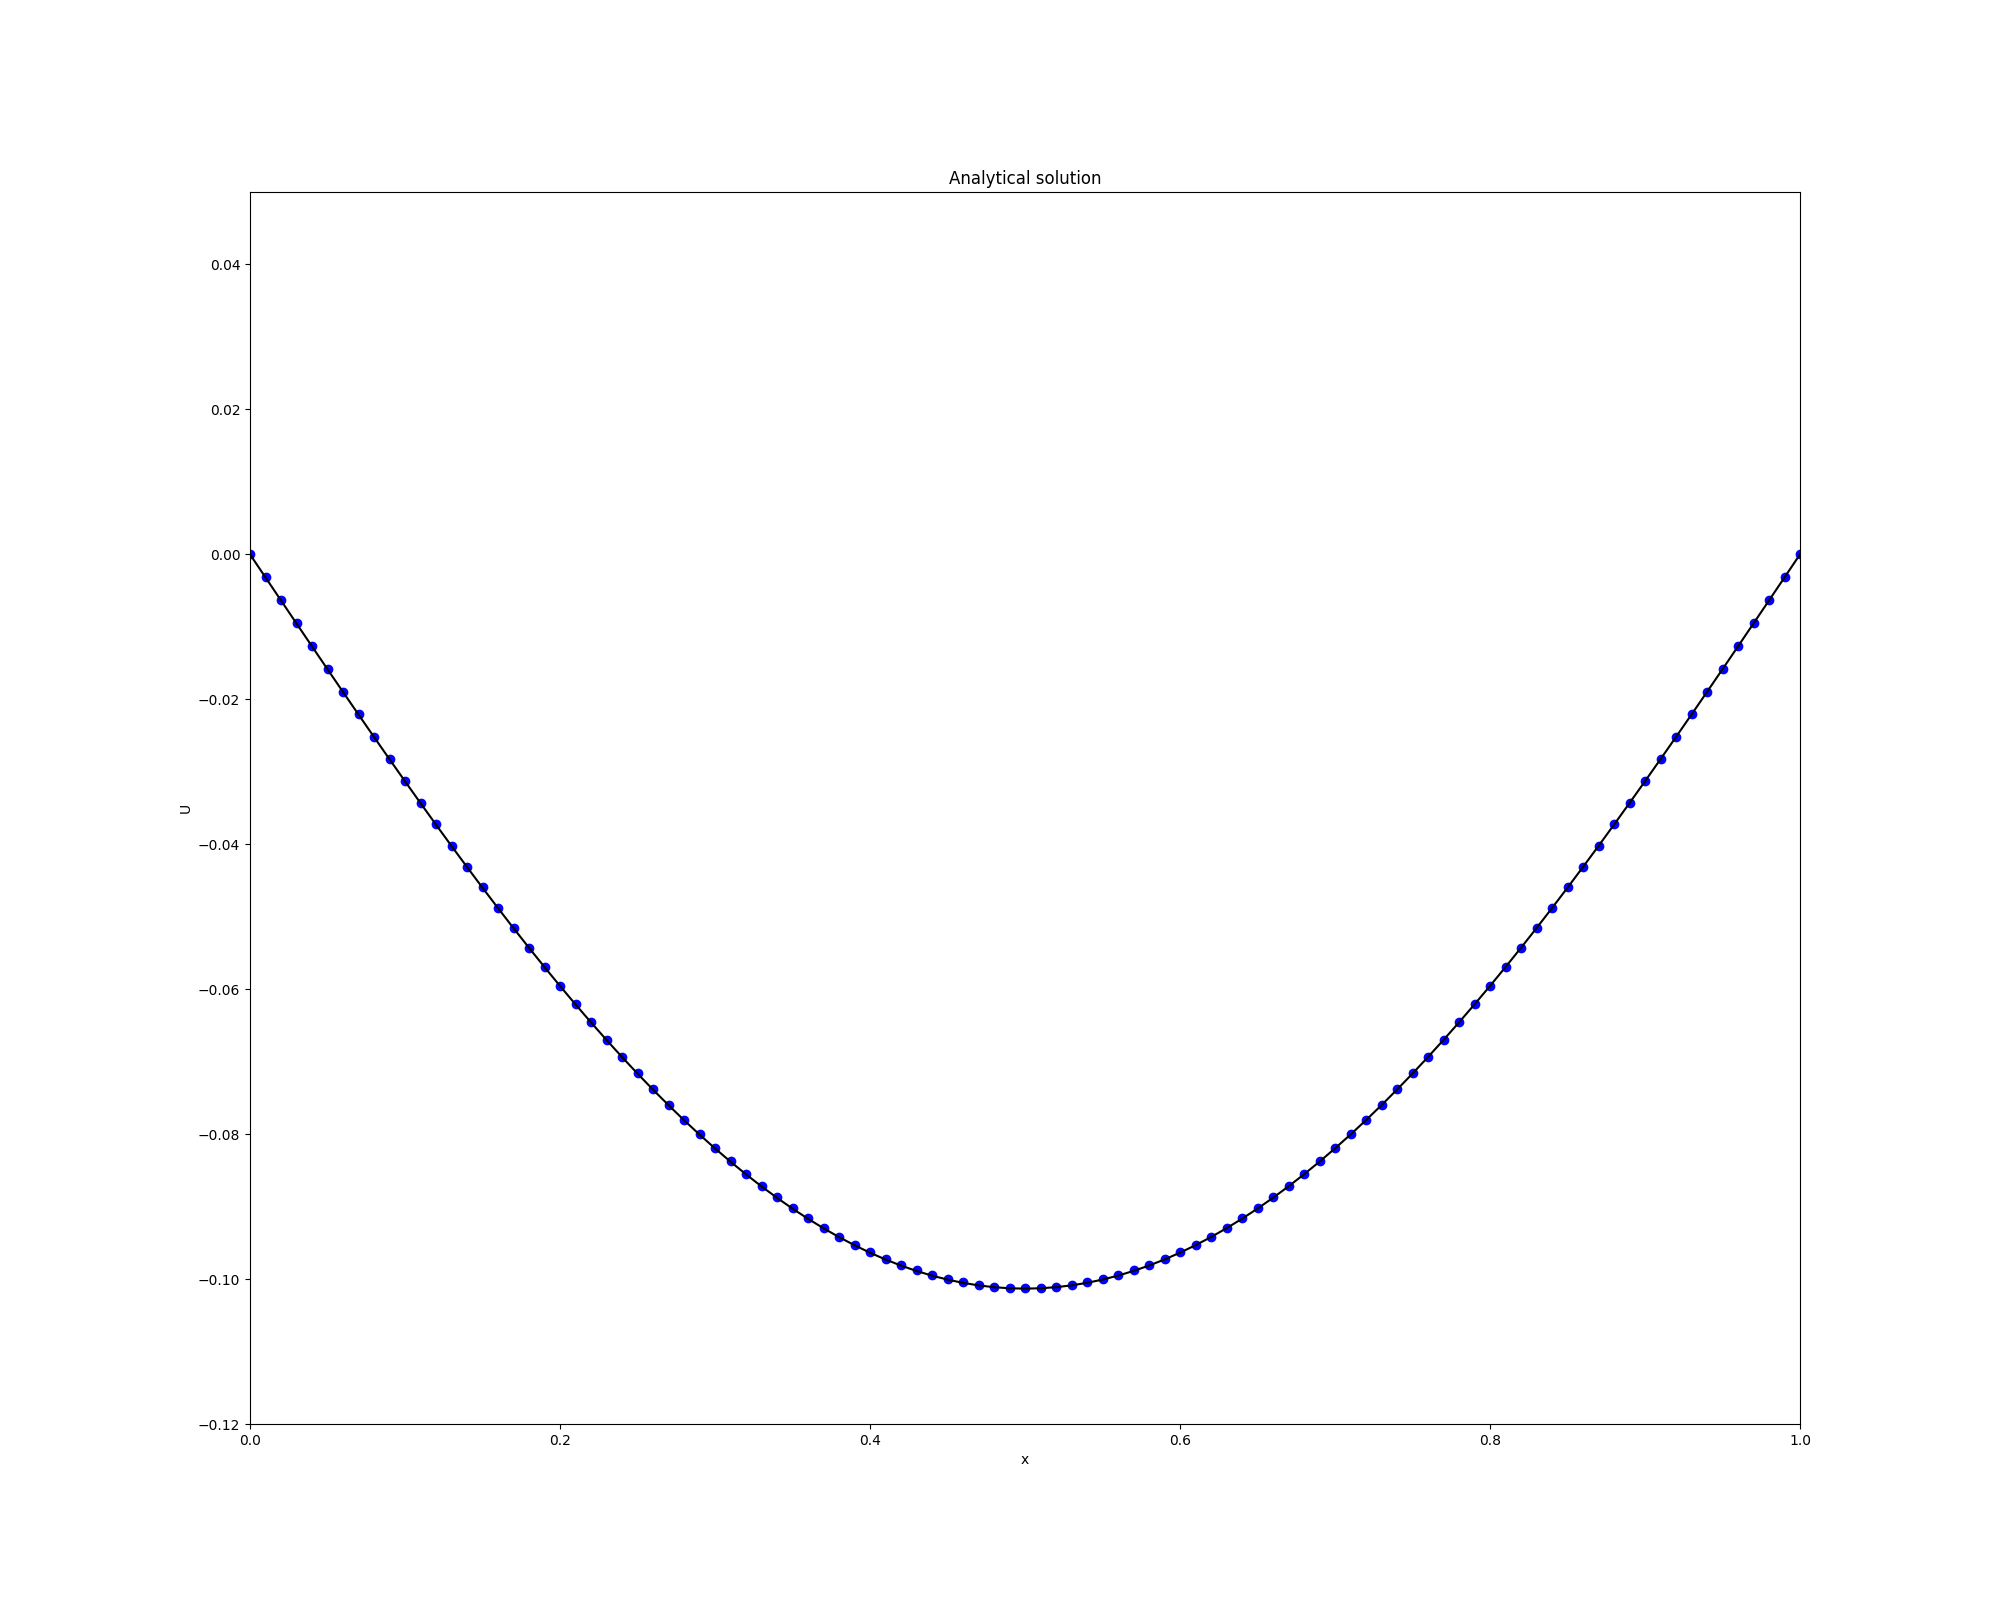
\includegraphics[width=0.5\textwidth, height=0.25\textwidth]{./image/Poisson_analytical.png}%
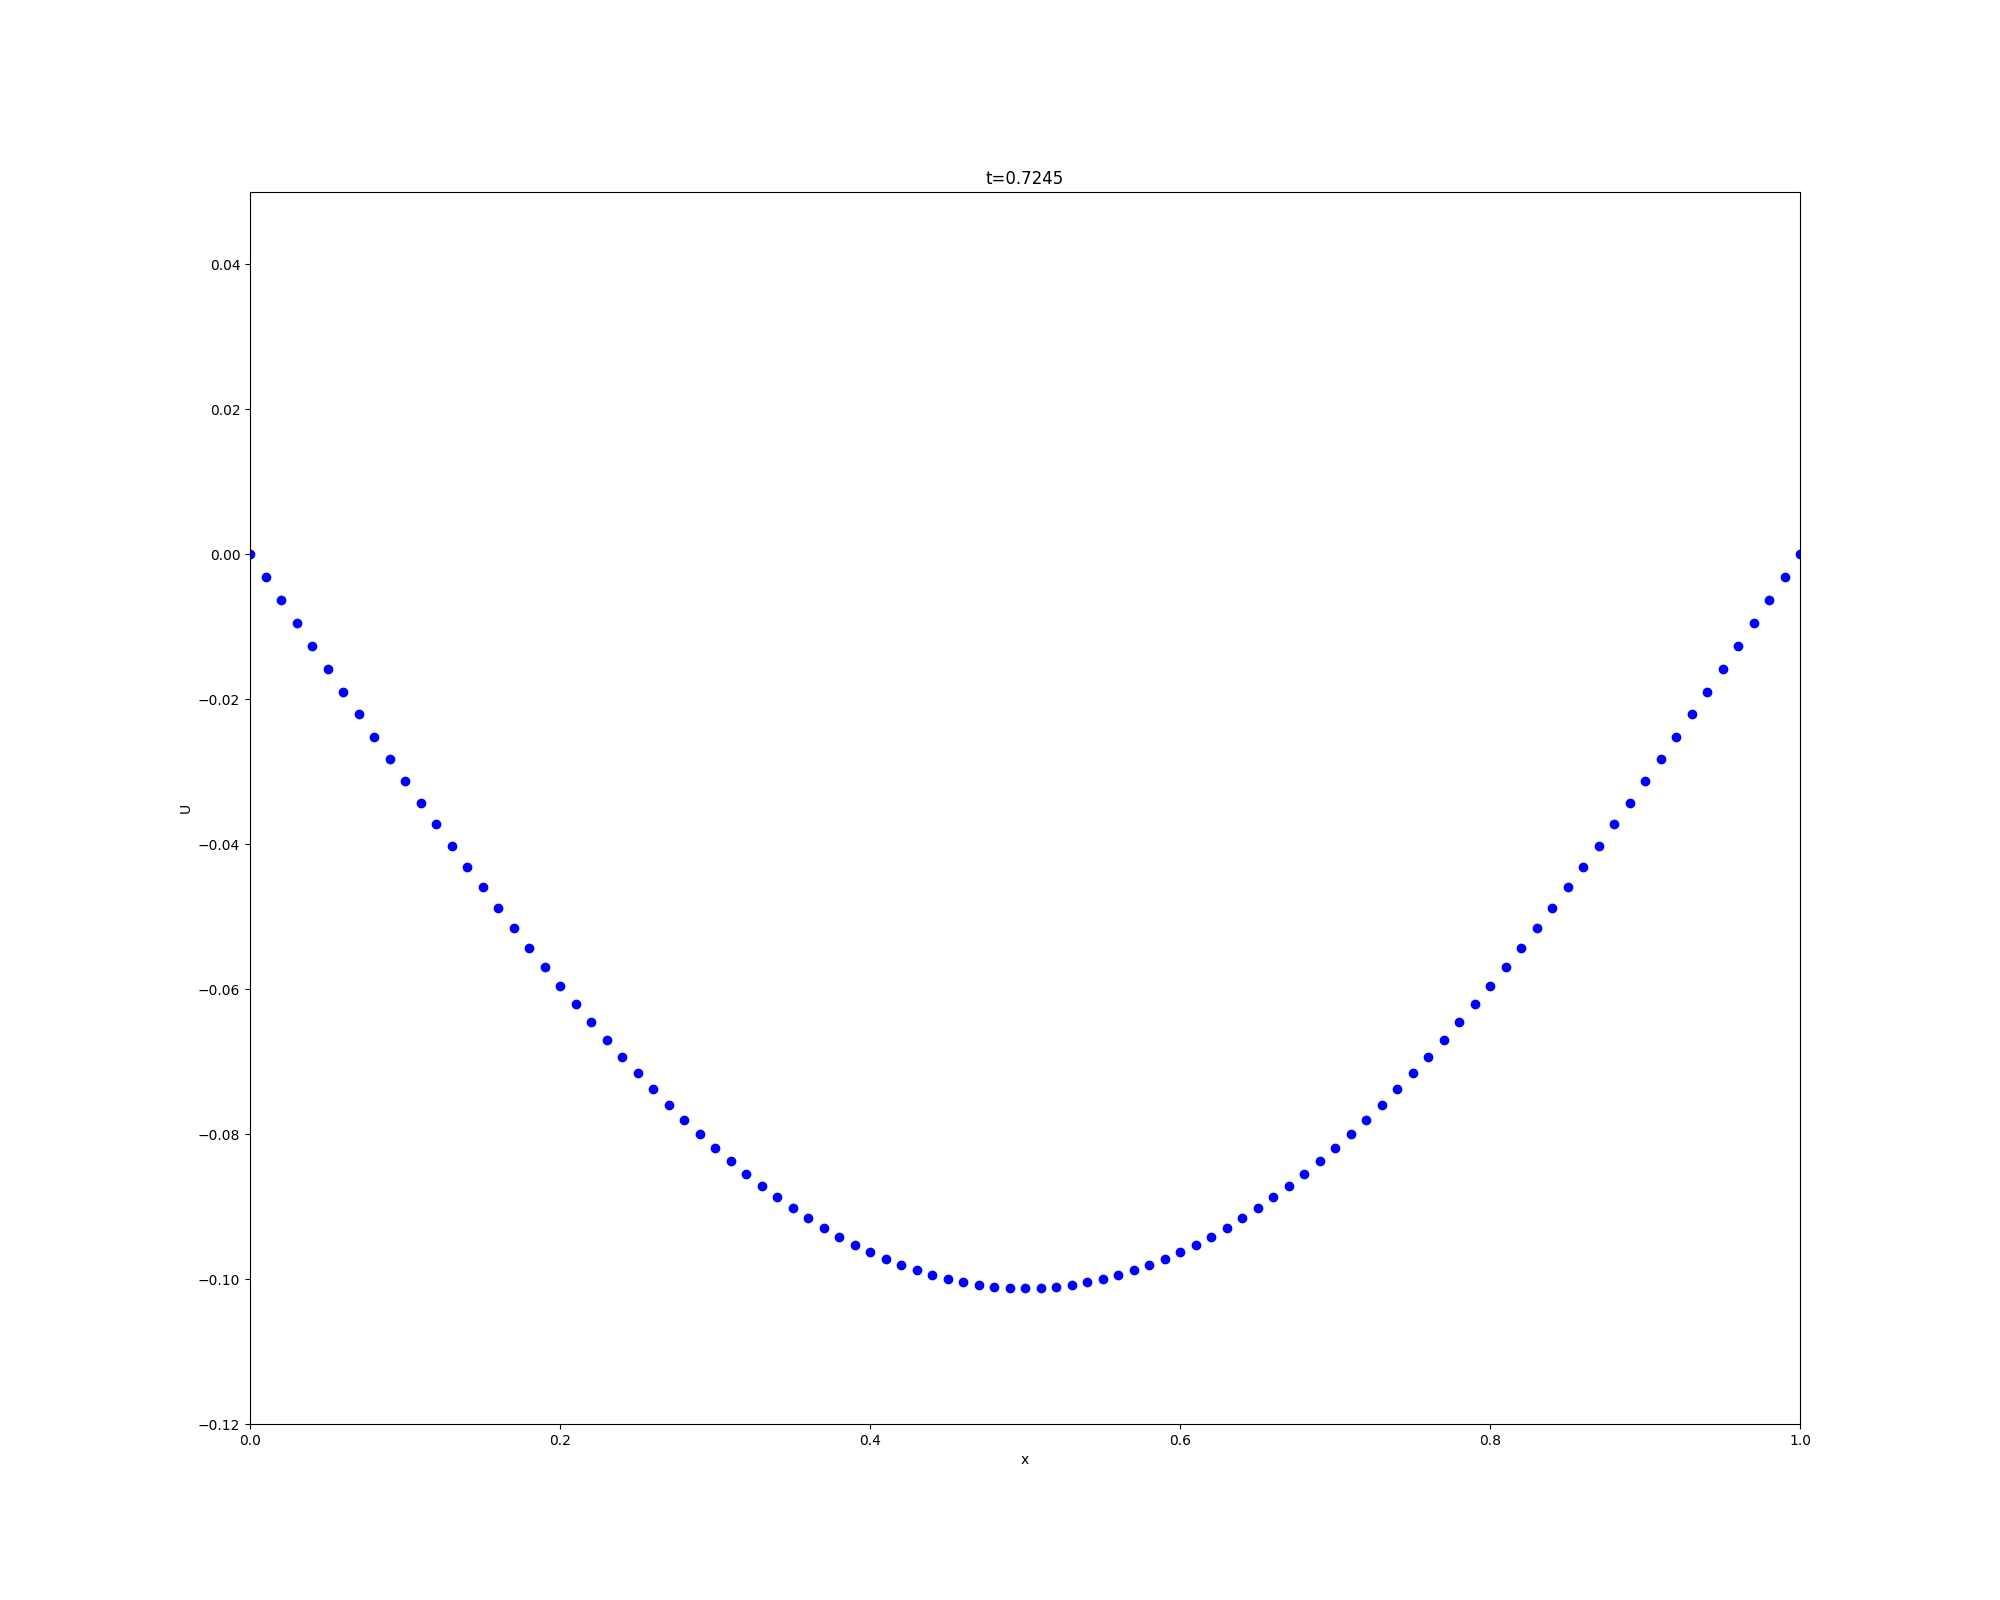
\includegraphics[width=0.5\textwidth, height=0.25\textwidth]{./image/Poisson_final_steps.png}
\caption{Left is comparison with analytical solution and right is the converged solution.}
\end{figure}
\end{itemize}
\end{frame}

\begin{frame}[fragile]
\PoissonTitle
\begin{itemize}
\item Sample of Poisson equation discretization in Python.
\lstinputlisting[language=Python, firstline=57, lastline=59]{./codes/Poisson1D.py}

\item The source term refers to $f\left(x\right)$

\end{itemize}
\end{frame}

\section{Finite Difference Method} 
\begin{frame}[fragile]
\frametitle{Standard template}
\begin{itemize}
\item This is a standard template slide.
\item Modify by adding items.
\end{itemize}

\end{frame}


%------------------------------------------------
\section{Finite Volume Method}
%------------------------------------------------

\begin{frame}[fragile]
\frametitle{Standard template}
\begin{itemize}
\item This is a standard template slide.
\item Modify by adding items.
\end{itemize}

\end{frame}


\section{Grid generation}

\begin{frame}[fragile]
\frametitle{Standard template}
\begin{itemize}
\item This is a standard template slide.
\item Modify by adding items.
\end{itemize}

\end{frame}


%\begin{frame}[fragile]
\frametitle{Standard template}
\begin{itemize}
\item This is a standard template slide.
\item Modify by adding items.
\end{itemize}

\end{frame}
\begin{frame}
\Huge{\centerline{Thank You!}}
\Huge{\centerline{Questions?}}
\end{frame}

\end{document} 